\documentclass{article}

%% Created with wxMaxima 16.04.2

\setlength{\parskip}{\medskipamount}
\setlength{\parindent}{0pt}
\usepackage[utf8]{inputenc}
\DeclareUnicodeCharacter{00B5}{\ensuremath{\mu}}
\usepackage{graphicx}
\usepackage{color}
\usepackage{amsmath}
\usepackage{ifthen}
\newsavebox{\picturebox}
\newlength{\pictureboxwidth}
\newlength{\pictureboxheight}
\newcommand{\includeimage}[1]{
    \savebox{\picturebox}{\includegraphics{#1}}
    \settoheight{\pictureboxheight}{\usebox{\picturebox}}
    \settowidth{\pictureboxwidth}{\usebox{\picturebox}}
    \ifthenelse{\lengthtest{\pictureboxwidth > .95\linewidth}}
    {
        \includegraphics[width=.95\linewidth,height=.80\textheight,keepaspectratio]{#1}
    }
    {
        \ifthenelse{\lengthtest{\pictureboxheight>.80\textheight}}
        {
            \includegraphics[width=.95\linewidth,height=.80\textheight,keepaspectratio]{#1}
            
        }
        {
            \includegraphics{#1}
        }
    }
}
\newlength{\thislabelwidth}
\DeclareMathOperator{\abs}{abs}
\usepackage{animate} % This package is required because the wxMaxima configuration option
                      % "Export animations to TeX" was enabled when this file was generated.

\definecolor{labelcolor}{RGB}{100,0,0}

\begin{document}

\pagebreak{}
{\Huge {\sc Mi tutorial de WXM
}}
\setcounter{section}{0}
\setcounter{subsection}{0}
\setcounter{figure}{0}


\section{Escritura
ctrl+1=agregar un nuevo text box
ctrl+2= agregar título principal
ctrl+3= agregar section
ctlr+4= agregar subsection
ctrl+5= agregar subsubsection}


\subsection{Arimética

}

para poder visualizar el resultado de una operación atirmética debemos presionar shift+enter 


\noindent
%%%%%%%%%%%%%%%
%%% INPUT:
\begin{minipage}[t]{8ex}\color{red}\bf
--\ensuremath{\ensuremath{>}}  
\end{minipage}
\begin{minipage}[t]{\textwidth}\color{blue}
 3+2;
\end{minipage}
%%% OUTPUT:
\[\displaystyle
\tag{\%{}o2}\label{o2} 
5\mbox{}
\]
%%%%%%%%%%%%%%%
punto y coma nos sirve para informar a máxima que el comando ha sido terminado por ejemplo, podemos tener diferentes comandos en una sola línea y el resultado de cada uno será expresado como una salida distinta 


\noindent
%%%%%%%%%%%%%%%
%%% INPUT:
\begin{minipage}[t]{8ex}\color{red}\bf
--\ensuremath{\ensuremath{>}}  
\end{minipage}
\begin{minipage}[t]{\textwidth}\color{blue}
3+8;5*3;sqrt(125);
\end{minipage}
%%% OUTPUT:
\[\displaystyle
\tag{\%{}o3}\label{o3} 
11\mbox{}\]
\[\displaystyle
\]
\[\tag{\%{}o4}\label{o4} 
15\mbox{}\]
\[\displaystyle
\]
\[\tag{\%{}o5}\label{o5} 
{{5}^{\frac{3}{2}}}\mbox{}
\]
%%%%%%%%%%%%%%%

\subsubsection{Uso de cálculos anteriores
}

Podemos observar que cada renglón, ya sea de entrada o salida está acompañado de un \% y la letra i u o indica si es entrada o salida así que podemos utilizar el nombre de la celda y llamardo 


\noindent
%%%%%%%%%%%%%%%
%%% INPUT:
\begin{minipage}[t]{8ex}\color{red}\bf
--\ensuremath{\ensuremath{>}}  
\end{minipage}
\begin{minipage}[t]{\textwidth}\color{blue}
(\%o4);
\end{minipage}
%%% OUTPUT:
\[\displaystyle
\tag{\%{}o9}\label{o9} 
15\mbox{}
\]
%%%%%%%%%%%%%%%


\noindent
%%%%%%%%%%%%%%%
%%% INPUT:
\begin{minipage}[t]{8ex}\color{red}\bf
--\ensuremath{\ensuremath{>}}  
\end{minipage}
\begin{minipage}[t]{\textwidth}\color{blue}
 (\%o4)*(\%o9);
\end{minipage}
%%% OUTPUT:
\[\displaystyle
\tag{\%{}o10}\label{o10} 
225\mbox{}
\]
%%%%%%%%%%%%%%%
incluso podemos realizar el cálculo pero ocultar la salida agregando un simbolo \$ al final 


\noindent
%%%%%%%%%%%%%%%
%%% INPUT:
\begin{minipage}[t]{8ex}\color{red}\bf
--\ensuremath{\ensuremath{>}}  
\end{minipage}
\begin{minipage}[t]{\textwidth}\color{blue}
 (\%o10)*5\$
\end{minipage}
y para visualizarlo, ponemos un \% y lo corremos, en la celda siguiente del cálculo 


\noindent
%%%%%%%%%%%%%%%
%%% INPUT:
\begin{minipage}[t]{8ex}\color{red}\bf
--\ensuremath{\ensuremath{>}}  
\end{minipage}
\begin{minipage}[t]{\textwidth}\color{blue}
 \%;
\end{minipage}
%%% OUTPUT:
\[\displaystyle
\tag{\%{}o16}\label{o16} 
1125\mbox{}
\]
%%%%%%%%%%%%%%%

\subsubsection{Observar la entrada de forma matemática
}

Podemos observar lo que introducimos como código a forma matemática agregando un apostrofe al inicio 


\noindent
%%%%%%%%%%%%%%%
%%% INPUT:
\begin{minipage}[t]{8ex}\color{red}\bf
--\ensuremath{\ensuremath{>}}  
\end{minipage}
\begin{minipage}[t]{\textwidth}\color{blue}
'(sqrt(32));
\end{minipage}
%%% OUTPUT:
\[\displaystyle
\tag{\%{}o18}\label{o18} 
{{2}^{\frac{5}{2}}}\mbox{}
\]
%%%%%%%%%%%%%%%


\noindent
%%%%%%%%%%%%%%%
%%% INPUT:
\begin{minipage}[t]{8ex}\color{red}\bf
--\ensuremath{\ensuremath{>}}  
\end{minipage}
\begin{minipage}[t]{\textwidth}\color{blue}
'integrate(x*sin(5*x),x);'limit(x*sin(5*x),x,5);
\end{minipage}
%%% OUTPUT:
\[\displaystyle
\tag{\%{}o27}\label{o27} 
\int {\left. x\,\sin{(5x)}dx\right.}\mbox{}\]
\[\displaystyle
\]
\[\tag{\%{}o28}\label{o28} 
\lim_{x\mbox{-\ensuremath{\ensuremath{>}}}5\to \mbox{-\ensuremath{\ensuremath{>}}}5}{x\,\sin{(5x)}}\mbox{}
\]
%%%%%%%%%%%%%%%

\subsubsection{Pedir decimales
}

Para poder expresar un valor con decimales debemos pedirle a maxima que lo realice con el comando float o si queremos restringir el número de decimales a mostrar utilizamos fpprintprec agregamos dos puntos y número de dígitos a mostrar y un simbolo \$ al final de este. 


\noindent
%%%%%%%%%%%%%%%
%%% INPUT:
\begin{minipage}[t]{8ex}\color{red}\bf
--\ensuremath{\ensuremath{>}}  
\end{minipage}
\begin{minipage}[t]{\textwidth}\color{blue}
 (31/4);
\end{minipage}
%%% OUTPUT:
\[\displaystyle
\tag{\%{}o29}\label{o29} 
\frac{31}{4}\mbox{}
\]
%%%%%%%%%%%%%%%


\noindent
%%%%%%%%%%%%%%%
%%% INPUT:
\begin{minipage}[t]{8ex}\color{red}\bf
--\ensuremath{\ensuremath{>}}  
\end{minipage}
\begin{minipage}[t]{\textwidth}\color{blue}
float(\%o29);
\end{minipage}
%%% OUTPUT:
\[\displaystyle
\tag{\%{}o30}\label{o30} 
7.75\mbox{}
\]
%%%%%%%%%%%%%%%


\noindent
%%%%%%%%%%%%%%%
%%% INPUT:
\begin{minipage}[t]{8ex}\color{red}\bf
--\ensuremath{\ensuremath{>}}  
\end{minipage}
\begin{minipage}[t]{\textwidth}\color{blue}
sqrt(3);
\end{minipage}
%%% OUTPUT:
\[\displaystyle
\tag{\%{}o31}\label{o31} 
\sqrt{3}\mbox{}
\]
%%%%%%%%%%%%%%%


\noindent
%%%%%%%%%%%%%%%
%%% INPUT:
\begin{minipage}[t]{8ex}\color{red}\bf
--\ensuremath{\ensuremath{>}}  
\end{minipage}
\begin{minipage}[t]{\textwidth}\color{blue}
float(\%o31);
\end{minipage}
%%% OUTPUT:
\[\displaystyle
\tag{\%{}o32}\label{o32} 
1.732050807568877\mbox{}
\]
%%%%%%%%%%%%%%%


\noindent
%%%%%%%%%%%%%%%
%%% INPUT:
\begin{minipage}[t]{8ex}\color{red}\bf
--\ensuremath{\ensuremath{>}}  
\end{minipage}
\begin{minipage}[t]{\textwidth}\color{blue}
fpprintprec:3\$ (\%o32);
\end{minipage}
%%% OUTPUT:
\[\displaystyle
\tag{\%{}o34}\label{o34} 
1.73\mbox{}
\]
%%%%%%%%%%%%%%%

\subsubsection{uso de e y pi
}

A lo que leí se usan de la siguiente manera ya que vienen de defecto en máxima, lo que sí se debe especificar con el número de decimales a mostar 


\noindent
%%%%%%%%%%%%%%%
%%% INPUT:
\begin{minipage}[t]{8ex}\color{red}\bf
--\ensuremath{\ensuremath{>}}  
\end{minipage}
\begin{minipage}[t]{\textwidth}\color{blue}
 \%e;float(\%e);
\end{minipage}
%%% OUTPUT:
\[\displaystyle
\tag{\%{}o36}\label{o36} 
\%{}e\mbox{}\]
\[\displaystyle
\]
\[\tag{\%{}o37}\label{o37} 
2.71\mbox{}
\]
%%%%%%%%%%%%%%%


\noindent
%%%%%%%%%%%%%%%
%%% INPUT:
\begin{minipage}[t]{8ex}\color{red}\bf
--\ensuremath{\ensuremath{>}}  
\end{minipage}
\begin{minipage}[t]{\textwidth}\color{blue}
fpprintprec:16\$ ;e;float(\%e);pi;float(\%pi);
\end{minipage}
%%% OUTPUT:
\[\displaystyle
\tag{\%{}o50}\label{o50} 
e\mbox{}\]
\[\displaystyle
\]
\[\tag{\%{}o51}\label{o51} 
2.718281828459045\mbox{}\]
\[\displaystyle
\]
\[\tag{\%{}o52}\label{o52} 
\pi\mbox{}\]
\[\displaystyle
\]
\[\tag{\%{}o53}\label{o53} 
3.141592653589793\mbox{}
\]
%%%%%%%%%%%%%%%

\subsubsection{Logaritmos
}

Recuerda que log(x) es el logaritmo natural, para relizar un cambio de base debes hacerlo manualmente 


\noindent
%%%%%%%%%%%%%%%
%%% INPUT:
\begin{minipage}[t]{8ex}\color{red}\bf
--\ensuremath{\ensuremath{>}}  
\end{minipage}
\begin{minipage}[t]{\textwidth}\color{blue}
 log(10)/log(2); float(log(10)/log(2));
\end{minipage}
%%% OUTPUT:
\[\displaystyle
\tag{\%{}o57}\label{o57} 
\frac{\log{(10)}}{\log{(2)}}\mbox{}\]
\[\displaystyle
\]
\[\tag{\%{}o58}\label{o58} 
3.321928094887362\mbox{}
\]
%%%%%%%%%%%%%%%
Puedes expandir los logaritmos (productos,sumas,cocientes,etc) por ejemplo antes de expandir 


\noindent
%%%%%%%%%%%%%%%
%%% INPUT:
\begin{minipage}[t]{8ex}\color{red}\bf
--\ensuremath{\ensuremath{>}}  
\end{minipage}
\begin{minipage}[t]{\textwidth}\color{blue}
 log(a*b\^{}2);
\end{minipage}
%%% OUTPUT:
\[\displaystyle
\tag{\%{}o72}\label{o72} 
\log{\left( a\,{{b}^{2}}\right) }\mbox{}
\]
%%%%%%%%%%%%%%%
usando logexpand 


\noindent
%%%%%%%%%%%%%%%
%%% INPUT:
\begin{minipage}[t]{8ex}\color{red}\bf
--\ensuremath{\ensuremath{>}}  
\end{minipage}
\begin{minipage}[t]{\textwidth}\color{blue}
 logexpand:super; log(a*b\^{}2);
\end{minipage}
%%% OUTPUT:
\[\displaystyle
\tag{logexpand}\label{logexpand}
\mathit{super}\mbox{}\]
\[\displaystyle
\]
\[\tag{\%{}o74}\label{o74} 
2\log{(b)}+\log{(a)}\mbox{}
\]
%%%%%%%%%%%%%%%
podemos desactivar el logexpand de la siguiente manera 


\noindent
%%%%%%%%%%%%%%%
%%% INPUT:
\begin{minipage}[t]{8ex}\color{red}\bf
--\ensuremath{\ensuremath{>}}  
\end{minipage}
\begin{minipage}[t]{\textwidth}\color{blue}
 logexpand:false; log(a*b\^{}2);
\end{minipage}
%%% OUTPUT:
\[\displaystyle
\tag{logexpand}\label{logexpand}
\mbox{false}\mbox{}\]
\[\displaystyle
\]
\[\tag{\%{}o76}\label{o76} 
\log{\left( a\,{{b}^{2}}\right) }\mbox{}
\]
%%%%%%%%%%%%%%%
 de igual manera se pueden contraer los logaritmos con logcontract 


\noindent
%%%%%%%%%%%%%%%
%%% INPUT:
\begin{minipage}[t]{8ex}\color{red}\bf
--\ensuremath{\ensuremath{>}}  
\end{minipage}
\begin{minipage}[t]{\textwidth}\color{blue}
    logcontract(log(a) + 2*log(b));
\end{minipage}
%%% OUTPUT:
\[\displaystyle
\tag{\%{}o77}\label{o77} 
\log{\left( a\,{{b}^{2}}\right) }\mbox{}
\]
%%%%%%%%%%%%%%%
el problema es que no funciona con coeficientes fraccionarios 

\subsubsection{Expansion de expresiones racionales}

podemos expresar algo como lo siguiente de forma desarrollada solo si se lo pedimos a maxima 


\noindent
%%%%%%%%%%%%%%%
%%% INPUT:
\begin{minipage}[t]{8ex}\color{red}\bf
--\ensuremath{\ensuremath{>}}  
\end{minipage}
\begin{minipage}[t]{\textwidth}\color{blue}
 (x+2)\^{}2;
\end{minipage}
%%% OUTPUT:
\[\displaystyle
\tag{\%{}o78}\label{o78} 
{{\left( x+2\right) }^{2}}\mbox{}
\]
%%%%%%%%%%%%%%%


\noindent
%%%%%%%%%%%%%%%
%%% INPUT:
\begin{minipage}[t]{8ex}\color{red}\bf
--\ensuremath{\ensuremath{>}}  
\end{minipage}
\begin{minipage}[t]{\textwidth}\color{blue}
 expand((x+2)\^{}2);
\end{minipage}
%%% OUTPUT:
\[\displaystyle
\tag{\%{}o79}\label{o79} 
{{x}^{2}}+4x+4\mbox{}
\]
%%%%%%%%%%%%%%%


\noindent
%%%%%%%%%%%%%%%
%%% INPUT:
\begin{minipage}[t]{8ex}\color{red}\bf
--\ensuremath{\ensuremath{>}}  
\end{minipage}
\begin{minipage}[t]{\textwidth}\color{blue}
 ((x+2)*(3*x-5)*(x-4)\^{}3);
\end{minipage}
%%% OUTPUT:
\[\displaystyle
\tag{\%{}o80}\label{o80} 
{{\left( x-4\right) }^{3}}\,\left( x+2\right) \,\left( 3x-5\right) \mbox{}
\]
%%%%%%%%%%%%%%%


\noindent
%%%%%%%%%%%%%%%
%%% INPUT:
\begin{minipage}[t]{8ex}\color{red}\bf
--\ensuremath{\ensuremath{>}}  
\end{minipage}
\begin{minipage}[t]{\textwidth}\color{blue}
 expand(\%i80);
\end{minipage}
%%% OUTPUT:
\[\displaystyle
\tag{\%{}o81}\label{o81} 
3{{x}^{5}}-35{{x}^{4}}+122{{x}^{3}}-24{{x}^{2}}-544x+640\mbox{}
\]
%%%%%%%%%%%%%%%
De igual forma se puede factorizar 


\noindent
%%%%%%%%%%%%%%%
%%% INPUT:
\begin{minipage}[t]{8ex}\color{red}\bf
--\ensuremath{\ensuremath{>}}  
\end{minipage}
\begin{minipage}[t]{\textwidth}\color{blue}
 factor(3*x\^{}5-35*x\^{}4+122*x\^{}3-24*x\^{}2-544*x+640);
\end{minipage}
%%% OUTPUT:
\[\displaystyle
\tag{\%{}o82}\label{o82} 
{{\left( x-4\right) }^{3}}\,\left( x+2\right) \,\left( 3x-5\right) \mbox{}
\]
%%%%%%%%%%%%%%%


\noindent
%%%%%%%%%%%%%%%
%%% INPUT:
\begin{minipage}[t]{8ex}\color{red}\bf
--\ensuremath{\ensuremath{>}}  
\end{minipage}
\begin{minipage}[t]{\textwidth}\color{blue}
 (1/(x+2)-(3*x+5)/(2-x)\^{}3);
\end{minipage}
%%% OUTPUT:
\[\displaystyle
\tag{\%{}o84}\label{o84} 
\frac{1}{x+2}-\frac{3x+5}{{{\left( 2-x\right) }^{3}}}\mbox{}
\]
%%%%%%%%%%%%%%%
también podemos factorizar pero en forma de fracción el ejemplo anterior puede ser factorizado de la siguiente forma 


\noindent
%%%%%%%%%%%%%%%
%%% INPUT:
\begin{minipage}[t]{8ex}\color{red}\bf
--\ensuremath{\ensuremath{>}}  
\end{minipage}
\begin{minipage}[t]{\textwidth}\color{blue}
 ratsimp((1/(x+2)-(3*x+5)/(2-x)\^{}3));
\end{minipage}
%%% OUTPUT:
\[\displaystyle
\tag{\%{}o85}\label{o85} 
\frac{{{x}^{3}}-3{{x}^{2}}+23x+2}{{{x}^{4}}-4{{x}^{3}}+16x-16}\mbox{}
\]
%%%%%%%%%%%%%%%
y podemos separarlos en denominador y numerador 


\noindent
%%%%%%%%%%%%%%%
%%% INPUT:
\begin{minipage}[t]{8ex}\color{red}\bf
--\ensuremath{\ensuremath{>}}  
\end{minipage}
\begin{minipage}[t]{\textwidth}\color{blue}
 denom(\%o85);num(\%o85);
\end{minipage}
%%% OUTPUT:
\[\displaystyle
\tag{\%{}o88}\label{o88} 
{{x}^{4}}-4{{x}^{3}}+16x-16\mbox{}\]
\[\displaystyle
\]
\[\tag{\%{}o89}\label{o89} 
{{x}^{3}}-3{{x}^{2}}+23x+2\mbox{}
\]
%%%%%%%%%%%%%%%

\subsection{Variables
}

Para dar valor a una variable dentro de una ecuación , la representamos con un signo igual. En cambio si queremos que el valor de la variable quede en la memoria de maxima debemos representarla con dos puntos 


\noindent
%%%%%%%%%%%%%%%
%%% INPUT:
\begin{minipage}[t]{8ex}\color{red}\bf
--\ensuremath{\ensuremath{>}}  
\end{minipage}
\begin{minipage}[t]{\textwidth}\color{blue}
 R=32;
\end{minipage}
%%% OUTPUT:
\[\displaystyle
\tag{\%{}o90}\label{o90} 
R=32\mbox{}
\]
%%%%%%%%%%%%%%%


\noindent
%%%%%%%%%%%%%%%
%%% INPUT:
\begin{minipage}[t]{8ex}\color{red}\bf
--\ensuremath{\ensuremath{>}}  
\end{minipage}
\begin{minipage}[t]{\textwidth}\color{blue}
R;
\end{minipage}
%%% OUTPUT:
\[\displaystyle
\tag{\%{}o91}\label{o91} 
R\mbox{}
\]
%%%%%%%%%%%%%%%


\noindent
%%%%%%%%%%%%%%%
%%% INPUT:
\begin{minipage}[t]{8ex}\color{red}\bf
--\ensuremath{\ensuremath{>}}  
\end{minipage}
\begin{minipage}[t]{\textwidth}\color{blue}
A:35;
\end{minipage}
%%% OUTPUT:
\[\displaystyle
\tag{A}\label{A}
35\mbox{}
\]
%%%%%%%%%%%%%%%


\noindent
%%%%%%%%%%%%%%%
%%% INPUT:
\begin{minipage}[t]{8ex}\color{red}\bf
--\ensuremath{\ensuremath{>}}  
\end{minipage}
\begin{minipage}[t]{\textwidth}\color{blue}
A;
\end{minipage}
%%% OUTPUT:
\[\displaystyle
\tag{\%{}o93}\label{o93} 
35\mbox{}
\]
%%%%%%%%%%%%%%%
Podemos eliminar las variables con el comando Kill 


\noindent
%%%%%%%%%%%%%%%
%%% INPUT:
\begin{minipage}[t]{8ex}\color{red}\bf
--\ensuremath{\ensuremath{>}}  
\end{minipage}
\begin{minipage}[t]{\textwidth}\color{blue}
 A;
\end{minipage}
%%% OUTPUT:
\[\displaystyle
\tag{\%{}o94}\label{o94} 
35\mbox{}
\]
%%%%%%%%%%%%%%%


\noindent
%%%%%%%%%%%%%%%
%%% INPUT:
\begin{minipage}[t]{8ex}\color{red}\bf
--\ensuremath{\ensuremath{>}}  
\end{minipage}
\begin{minipage}[t]{\textwidth}\color{blue}
kill(A);
\end{minipage}
%%% OUTPUT:
\[\displaystyle
\tag{\%{}o95}\label{o95} 
\mathit{done}\mbox{}
\]
%%%%%%%%%%%%%%%


\noindent
%%%%%%%%%%%%%%%
%%% INPUT:
\begin{minipage}[t]{8ex}\color{red}\bf
--\ensuremath{\ensuremath{>}}  
\end{minipage}
\begin{minipage}[t]{\textwidth}\color{blue}
A;
\end{minipage}
%%% OUTPUT:
\[\displaystyle
\tag{\%{}o96}\label{o96} 
A\mbox{}
\]
%%%%%%%%%%%%%%%

\subsection{Funciones
}

Para Definir una función utilizamos dos puntos y un signo igual 


\noindent
%%%%%%%%%%%%%%%
%%% INPUT:
\begin{minipage}[t]{8ex}\color{red}\bf
--\ensuremath{\ensuremath{>}}  
\end{minipage}
\begin{minipage}[t]{\textwidth}\color{blue}
f(x):2*x+5;
\end{minipage}
%%% OUTPUT:
\[\displaystyle
\mbox{}\\\mbox{assignment: cannot assign to }\operatorname{f}(x)\mbox{ -- an error. To debug this try: debugmode(true);}\mbox{}
\]
%%%%%%%%%%%%%%%


\noindent
%%%%%%%%%%%%%%%
%%% INPUT:
\begin{minipage}[t]{8ex}\color{red}\bf
--\ensuremath{\ensuremath{>}}  
\end{minipage}
\begin{minipage}[t]{\textwidth}\color{blue}
 f(x):=2*x+5;
\end{minipage}
%%% OUTPUT:
\[\displaystyle
\tag{\%{}o98}\label{o98} 
\operatorname{f}(x):=2x+5\mbox{}
\]
%%%%%%%%%%%%%%%


\noindent
%%%%%%%%%%%%%%%
%%% INPUT:
\begin{minipage}[t]{8ex}\color{red}\bf
--\ensuremath{\ensuremath{>}}  
\end{minipage}
\begin{minipage}[t]{\textwidth}\color{blue}
 f(x);
\end{minipage}
%%% OUTPUT:
\[\displaystyle
\tag{\%{}o99}\label{o99} 
2x+5\mbox{}
\]
%%%%%%%%%%%%%%%
 las evaluamos de la siguiente manera Ponemos el valor que va a tomar la la variable x en la función y listo. 


\noindent
%%%%%%%%%%%%%%%
%%% INPUT:
\begin{minipage}[t]{8ex}\color{red}\bf
--\ensuremath{\ensuremath{>}}  
\end{minipage}
\begin{minipage}[t]{\textwidth}\color{blue}
f(5);f(\%pi);f(sqrt(2));
\end{minipage}
%%% OUTPUT:
\[\displaystyle
\tag{\%{}o100}\label{o100} 
15\mbox{}\]
\[\displaystyle
\]
\[\tag{\%{}o101}\label{o101} 
2\ensuremath{\pi} +5\mbox{}\]
\[\displaystyle
\]
\[\tag{\%{}o102}\label{o102} 
{{2}^{\frac{3}{2}}}+5\mbox{}
\]
%%%%%%%%%%%%%%%
Tenemos la ventaja de que podemos usar cualquier variable dentro de la función También podemos hacer mención acerca de la composición en maxima, esta es muy buena y correcta. 


\noindent
%%%%%%%%%%%%%%%
%%% INPUT:
\begin{minipage}[t]{8ex}\color{red}\bf
--\ensuremath{\ensuremath{>}}  
\end{minipage}
\begin{minipage}[t]{\textwidth}\color{blue}
 g(z):=sin(z)/(log(z)+z\^{}2);
\end{minipage}
%%% OUTPUT:
\[\displaystyle
\tag{\%{}o105}\label{o105} 
\operatorname{g}(z):=\frac{\sin{(z)}}{\log{(z)}+{{z}^{2}}}\mbox{}
\]
%%%%%%%%%%%%%%%


\noindent
%%%%%%%%%%%%%%%
%%% INPUT:
\begin{minipage}[t]{8ex}\color{red}\bf
--\ensuremath{\ensuremath{>}}  
\end{minipage}
\begin{minipage}[t]{\textwidth}\color{blue}
 g(\%pi);g(2);
\end{minipage}
%%% OUTPUT:
\[\displaystyle
\tag{\%{}o106}\label{o106} 
0\mbox{}\]
\[\displaystyle
\]
\[\tag{\%{}o107}\label{o107} 
\frac{\sin{(2)}}{\log{(2)}+4}\mbox{}
\]
%%%%%%%%%%%%%%%


\noindent
%%%%%%%%%%%%%%%
%%% INPUT:
\begin{minipage}[t]{8ex}\color{red}\bf
--\ensuremath{\ensuremath{>}}  
\end{minipage}
\begin{minipage}[t]{\textwidth}\color{blue}
	f(x):=3*x\^{}2+10; h(x):=g(f(x));
\end{minipage}
%%% OUTPUT:
\[\displaystyle
\tag{\%{}o113}\label{o113} 
\operatorname{f}(x):=3{{x}^{2}}+10\mbox{}\]
\[\displaystyle
\]
\[\tag{\%{}o114}\label{o114} 
\operatorname{h}(x):=\operatorname{g}\left( \operatorname{f}(x)\right) \mbox{}
\]
%%%%%%%%%%%%%%%


\noindent
%%%%%%%%%%%%%%%
%%% INPUT:
\begin{minipage}[t]{8ex}\color{red}\bf
--\ensuremath{\ensuremath{>}}  
\end{minipage}
\begin{minipage}[t]{\textwidth}\color{blue}
h(x);
\end{minipage}
%%% OUTPUT:
\[\displaystyle
\tag{\%{}o112}\label{o112} 
\frac{\sin{\left( 3{{x}^{2}}+10\right) }}{\log{\left( 3{{x}^{2}}+10\right) }+{{\left( 3{{x}^{2}}+10\right) }^{2}}}\mbox{}
\]
%%%%%%%%%%%%%%%

\subsection{Ecuaciones}


\subsubsection{Definir y trabajar con ecuaciones}

Para definir una ecuación damos la variable que va identificar a esta, dos puntos para asignar valores y el simbolo igual para mostrar la igualdad, por ejemplo. 


\noindent
%%%%%%%%%%%%%%%
%%% INPUT:
\begin{minipage}[t]{8ex}\color{red}\bf
--\ensuremath{\ensuremath{>}}  
\end{minipage}
\begin{minipage}[t]{\textwidth}\color{blue}
 Q:x\^{}3=5;
\end{minipage}
%%% OUTPUT:
\[\displaystyle
\tag{Q}\label{Q}
{{x}^{3}}=5\mbox{}
\]
%%%%%%%%%%%%%%%


\noindent
%%%%%%%%%%%%%%%
%%% INPUT:
\begin{minipage}[t]{8ex}\color{red}\bf
--\ensuremath{\ensuremath{>}}  
\end{minipage}
\begin{minipage}[t]{\textwidth}\color{blue}
Q;
\end{minipage}
%%% OUTPUT:
\[\displaystyle
\tag{\%{}o2}\label{o2} 
{{x}^{3}}=5\mbox{}
\]
%%%%%%%%%%%%%%%


\noindent
%%%%%%%%%%%%%%%
%%% INPUT:
\begin{minipage}[t]{8ex}\color{red}\bf
--\ensuremath{\ensuremath{>}}  
\end{minipage}
\begin{minipage}[t]{\textwidth}\color{blue}
R: x\^{}6+6=21;
\end{minipage}
%%% OUTPUT:
\[\displaystyle
\tag{R}\label{R}
{{x}^{6}}+6=21\mbox{}
\]
%%%%%%%%%%%%%%%


\noindent
%%%%%%%%%%%%%%%
%%% INPUT:
\begin{minipage}[t]{8ex}\color{red}\bf
--\ensuremath{\ensuremath{>}}  
\end{minipage}
\begin{minipage}[t]{\textwidth}\color{blue}
 R;
\end{minipage}
%%% OUTPUT:
\[\displaystyle
\tag{\%{}o4}\label{o4} 
{{x}^{6}}+6=21\mbox{}
\]
%%%%%%%%%%%%%%%
Podemos realizar operaciones con dos ecuaciones, así como sumar,multiplicar 


\noindent
%%%%%%%%%%%%%%%
%%% INPUT:
\begin{minipage}[t]{8ex}\color{red}\bf
--\ensuremath{\ensuremath{>}}  
\end{minipage}
\begin{minipage}[t]{\textwidth}\color{blue}
 Q+R;
\end{minipage}
%%% OUTPUT:
\[\displaystyle
\tag{\%{}o5}\label{o5} 
{{x}^{6}}+{{x}^{3}}+6=26\mbox{}
\]
%%%%%%%%%%%%%%%


\noindent
%%%%%%%%%%%%%%%
%%% INPUT:
\begin{minipage}[t]{8ex}\color{red}\bf
--\ensuremath{\ensuremath{>}}  
\end{minipage}
\begin{minipage}[t]{\textwidth}\color{blue}
 Q\^{}2;
\end{minipage}
%%% OUTPUT:
\[\displaystyle
\tag{\%{}o6}\label{o6} 
{{x}^{6}}=25\mbox{}
\]
%%%%%%%%%%%%%%%


\noindent
%%%%%%%%%%%%%%%
%%% INPUT:
\begin{minipage}[t]{8ex}\color{red}\bf
--\ensuremath{\ensuremath{>}}  
\end{minipage}
\begin{minipage}[t]{\textwidth}\color{blue}
sqrt(R)-sqrt(Q);
\end{minipage}
%%% OUTPUT:
\[\displaystyle
\tag{\%{}o7}\label{o7} 
\sqrt{{{x}^{6}}+6}-{{x}^{\frac{3}{2}}}=\sqrt{21}-\sqrt{5}\mbox{}
\]
%%%%%%%%%%%%%%%
También podemos solicitar que se nos muestre solo una parte de la ecuación, ya sea la parte derecha(rhs) o la parte izquierda(lhs). 


\noindent
%%%%%%%%%%%%%%%
%%% INPUT:
\begin{minipage}[t]{8ex}\color{red}\bf
--\ensuremath{\ensuremath{>}}  
\end{minipage}
\begin{minipage}[t]{\textwidth}\color{blue}
 H:y\^{}2+2=x\^{}4-5;
\end{minipage}
%%% OUTPUT:
\[\displaystyle
\tag{H}\label{H}
{{y}^{2}}+2={{x}^{4}}-5\mbox{}
\]
%%%%%%%%%%%%%%%


\noindent
%%%%%%%%%%%%%%%
%%% INPUT:
\begin{minipage}[t]{8ex}\color{red}\bf
--\ensuremath{\ensuremath{>}}  
\end{minipage}
\begin{minipage}[t]{\textwidth}\color{blue}
rhs(H);
\end{minipage}
%%% OUTPUT:
\[\displaystyle
\tag{\%{}o9}\label{o9} 
{{x}^{4}}-5\mbox{}
\]
%%%%%%%%%%%%%%%


\noindent
%%%%%%%%%%%%%%%
%%% INPUT:
\begin{minipage}[t]{8ex}\color{red}\bf
--\ensuremath{\ensuremath{>}}  
\end{minipage}
\begin{minipage}[t]{\textwidth}\color{blue}
 lhs(H);
\end{minipage}
%%% OUTPUT:
\[\displaystyle
\tag{\%{}o10}\label{o10} 
{{y}^{2}}+2\mbox{}
\]
%%%%%%%%%%%%%%%

\subsubsection{Resolver Ecuaciones}

Para resolver ecuaciones utilizamos solve(ecuación,variable) 


\noindent
%%%%%%%%%%%%%%%
%%% INPUT:
\begin{minipage}[t]{8ex}\color{red}\bf
--\ensuremath{\ensuremath{>}}  
\end{minipage}
\begin{minipage}[t]{\textwidth}\color{blue}
 solve(5*x\^{}3=125,x);
\end{minipage}
%%% OUTPUT:
\[\displaystyle
\tag{\%{}o1}\label{o1} 
[x=\frac{\sqrt{3}\,{{25}^{\frac{1}{3}}}\%{}i-{{25}^{\frac{1}{3}}}}{2},x=-\frac{\sqrt{3}\,{{25}^{\frac{1}{3}}}\%{}i+{{25}^{\frac{1}{3}}}}{2},x={{25}^{\frac{1}{3}}}]\mbox{}
\]
%%%%%%%%%%%%%%%
Podemos resolver ecuaciones de varias variables y solo especificar en términos de que variable queremos que quede. 


\noindent
%%%%%%%%%%%%%%%
%%% INPUT:
\begin{minipage}[t]{8ex}\color{red}\bf
--\ensuremath{\ensuremath{>}}  
\end{minipage}
\begin{minipage}[t]{\textwidth}\color{blue}
 solve(Q=3*(xy+y\^{}2),y);
\end{minipage}
%%% OUTPUT:
\[\displaystyle
\tag{\%{}o2}\label{o2} 
[y=-\frac{\sqrt{Q-3\mathit{xy}}}{\sqrt{3}},y=\frac{\sqrt{Q-3\mathit{xy}}}{\sqrt{3}}]\mbox{}
\]
%%%%%%%%%%%%%%%


\noindent
%%%%%%%%%%%%%%%
%%% INPUT:
\begin{minipage}[t]{8ex}\color{red}\bf
--\ensuremath{\ensuremath{>}}  
\end{minipage}
\begin{minipage}[t]{\textwidth}\color{blue}
 solve(Y=2*(X+W)/(Z),Z);
\end{minipage}
%%% OUTPUT:
\[\displaystyle
\tag{\%{}o5}\label{o5} 
[Z=\frac{2X+2W}{Y}]\mbox{}
\]
%%%%%%%%%%%%%%%
También podemos resolver un función. 


\noindent
%%%%%%%%%%%%%%%
%%% INPUT:
\begin{minipage}[t]{8ex}\color{red}\bf
--\ensuremath{\ensuremath{>}}  
\end{minipage}
\begin{minipage}[t]{\textwidth}\color{blue}
 f(x):=3*x\^{}2-2*x;
\end{minipage}
%%% OUTPUT:
\[\displaystyle
\tag{\%{}o6}\label{o6} 
\operatorname{f}(x):=3{{x}^{2}}-2x\mbox{}
\]
%%%%%%%%%%%%%%%


\noindent
%%%%%%%%%%%%%%%
%%% INPUT:
\begin{minipage}[t]{8ex}\color{red}\bf
--\ensuremath{\ensuremath{>}}  
\end{minipage}
\begin{minipage}[t]{\textwidth}\color{blue}
solve(f(x)=21,x);
\end{minipage}
%%% OUTPUT:
\[\displaystyle
\tag{\%{}o7}\label{o7} 
[x=-\frac{7}{3},x=3]\mbox{}
\]
%%%%%%%%%%%%%%%


\noindent
%%%%%%%%%%%%%%%
%%% INPUT:
\begin{minipage}[t]{8ex}\color{red}\bf
--\ensuremath{\ensuremath{>}}  
\end{minipage}
\begin{minipage}[t]{\textwidth}\color{blue}
f(x);
\end{minipage}
%%% OUTPUT:
\[\displaystyle
\tag{\%{}o8}\label{o8} 
3{{x}^{2}}-2x\mbox{}
\]
%%%%%%%%%%%%%%%


\noindent
%%%%%%%%%%%%%%%
%%% INPUT:
\begin{minipage}[t]{8ex}\color{red}\bf
--\ensuremath{\ensuremath{>}}  
\end{minipage}
\begin{minipage}[t]{\textwidth}\color{blue}
f(x);g(x)=1/(x\^{}2+1);
\end{minipage}
%%% OUTPUT:
\[\displaystyle
\tag{\%{}o10}\label{o10} 
3{{x}^{2}}-2x\mbox{}\]
\[\displaystyle
\]
\[\tag{\%{}o11}\label{o11} 
\operatorname{g}(x)=\frac{1}{{{x}^{2}}+1}\mbox{}
\]
%%%%%%%%%%%%%%%


\noindent
%%%%%%%%%%%%%%%
%%% INPUT:
\begin{minipage}[t]{8ex}\color{red}\bf
--\ensuremath{\ensuremath{>}}  
\end{minipage}
\begin{minipage}[t]{\textwidth}\color{blue}
f(g(x)),x;
\end{minipage}
%%% OUTPUT:
\[\displaystyle
\tag{\%{}o12}\label{o12} 
3{{\operatorname{g}(x)}^{2}}-2\operatorname{g}(x)\mbox{}
\]
%%%%%%%%%%%%%%%


\noindent
%%%%%%%%%%%%%%%
%%% INPUT:
\begin{minipage}[t]{8ex}\color{red}\bf
--\ensuremath{\ensuremath{>}}  
\end{minipage}
\begin{minipage}[t]{\textwidth}\color{blue}
solve(f(x)=g(f(x)),x);
\end{minipage}
%%% OUTPUT:
\[\displaystyle
\tag{\%{}o13}\label{o13} 
[x=-\frac{\sqrt{3\operatorname{g}\left( 3{{x}^{2}}-2x\right) +1}-1}{3},x=\frac{\sqrt{3\operatorname{g}\left( 3{{x}^{2}}-2x\right) +1}+1}{3}]\mbox{}
\]
%%%%%%%%%%%%%%%


\noindent
%%%%%%%%%%%%%%%
%%% INPUT:
\begin{minipage}[t]{8ex}\color{red}\bf
--\ensuremath{\ensuremath{>}}  
\end{minipage}
\begin{minipage}[t]{\textwidth}\color{blue}
 kill(f,g);
\end{minipage}
%%% OUTPUT:
\[\displaystyle
\tag{\%{}o14}\label{o14} 
\mathit{done}\mbox{}
\]
%%%%%%%%%%%%%%%


\noindent
%%%%%%%%%%%%%%%
%%% INPUT:
\begin{minipage}[t]{8ex}\color{red}\bf
--\ensuremath{\ensuremath{>}}  
\end{minipage}
\begin{minipage}[t]{\textwidth}\color{blue}
f(x);
\end{minipage}
%%% OUTPUT:
\[\displaystyle
\tag{\%{}o15}\label{o15} 
\operatorname{f}(x)\mbox{}
\]
%%%%%%%%%%%%%%%


\noindent
%%%%%%%%%%%%%%%
%%% INPUT:
\begin{minipage}[t]{8ex}\color{red}\bf
--\ensuremath{\ensuremath{>}}  
\end{minipage}
\begin{minipage}[t]{\textwidth}\color{blue}

\end{minipage}
Recuerda que si ponemos solve seguido de una función la resolverá para f(x)=0 

\subsection{Ploteo}

Ahora veremos un poco acerca de cómo graficar 
Empezaremos por graficar en 2D, para ello necesitamos el comando wxplot2d(funcion,[dominio]) 


\noindent
%%%%%%%%%%%%%%%
%%% INPUT:
\begin{minipage}[t]{8ex}\color{red}\bf
--\ensuremath{\ensuremath{>}}  
\end{minipage}
\begin{minipage}[t]{\textwidth}\color{blue}
 wxplot2d(x\^{}2+1,[x,0,5]);
\end{minipage}
%%% OUTPUT:
\[\displaystyle
\tag{\%{}t30}\label{t30} 
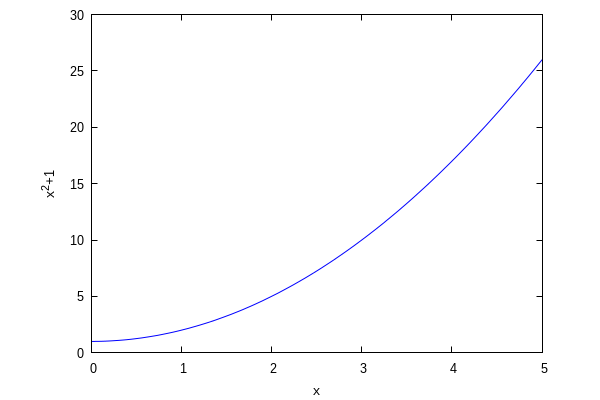
\includegraphics[width=.95\linewidth,height=.80\textheight,keepaspectratio]{Trabajoclase_img/Trabajoclase_1}\mbox{}\]
\[\displaystyle
\]
\[\tag{\%{}o30}\label{o30} 
\mbox{}
\]
%%%%%%%%%%%%%%%


\noindent
%%%%%%%%%%%%%%%
%%% INPUT:
\begin{minipage}[t]{8ex}\color{red}\bf
--\ensuremath{\ensuremath{>}}  
\end{minipage}
\begin{minipage}[t]{\textwidth}\color{blue}
 f(x):=3*x\^{}3 - 5*x\^{}2;
wxplot2d(f(x),[x,-2,2]);
\end{minipage}
%%% OUTPUT:
\[\displaystyle
\tag{\%{}o31}\label{o31} 
\operatorname{f}(x):=3{{x}^{3}}-5{{x}^{2}}\mbox{}\]
\[\displaystyle
\]
\[\tag{\%{}t32}\label{t32} 
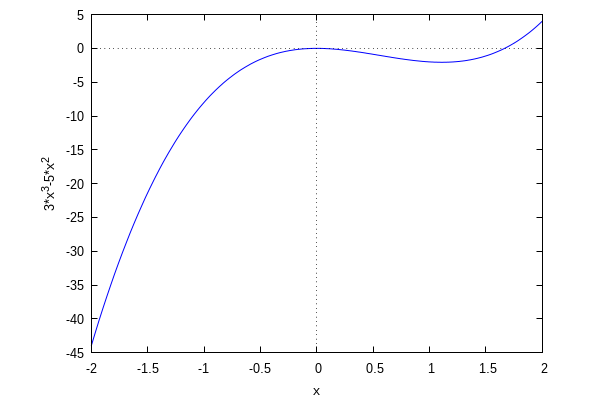
\includegraphics[width=.95\linewidth,height=.80\textheight,keepaspectratio]{Trabajoclase_img/Trabajoclase_2}\mbox{}\]
\[\displaystyle
\]
\[\tag{\%{}o32}\label{o32} 
\mbox{}
\]
%%%%%%%%%%%%%%%
También podemos graficar varias funciones en el mismo eje. utilizamos wxplot2d([f1,f2,...,fn],[eje de límite,liminf,limsup]) 


\noindent
%%%%%%%%%%%%%%%
%%% INPUT:
\begin{minipage}[t]{8ex}\color{red}\bf
--\ensuremath{\ensuremath{>}}  
\end{minipage}
\begin{minipage}[t]{\textwidth}\color{blue}
 wxplot2d([f(x),2-5*x\^{}2],[x,-2,2]);
\end{minipage}
%%% OUTPUT:
\[\displaystyle
\tag{\%{}t33}\label{t33} 
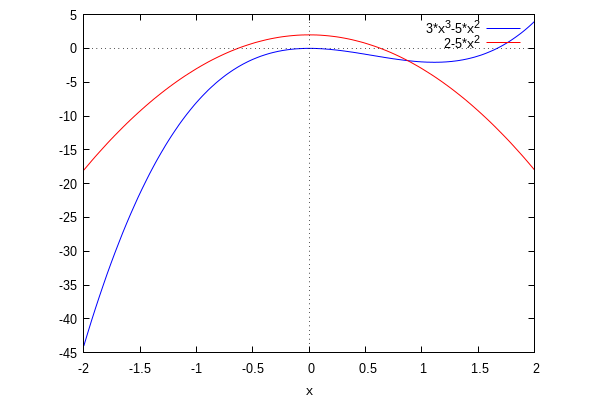
\includegraphics[width=.95\linewidth,height=.80\textheight,keepaspectratio]{Trabajoclase_img/Trabajoclase_3}\mbox{}\]
\[\displaystyle
\]
\[\tag{\%{}o33}\label{o33} 
\mbox{}
\]
%%%%%%%%%%%%%%%
Podemos también agregar la legenda  a las gráficas. utilizamos el mismo comando solo que ahora después del dominio agregamos [legend,"nombre1","nombre2","nombre3",...,"nombren"] 


\noindent
%%%%%%%%%%%%%%%
%%% INPUT:
\begin{minipage}[t]{8ex}\color{red}\bf
--\ensuremath{\ensuremath{>}}  
\end{minipage}
\begin{minipage}[t]{\textwidth}\color{blue}
wxplot2d([x\^{}2,3*x\^{}2,5*x\^{}2],[x,-2,2],[legend,"One","Three","Five"]);
\end{minipage}
%%% OUTPUT:
\[\displaystyle
\tag{\%{}t34}\label{t34} 
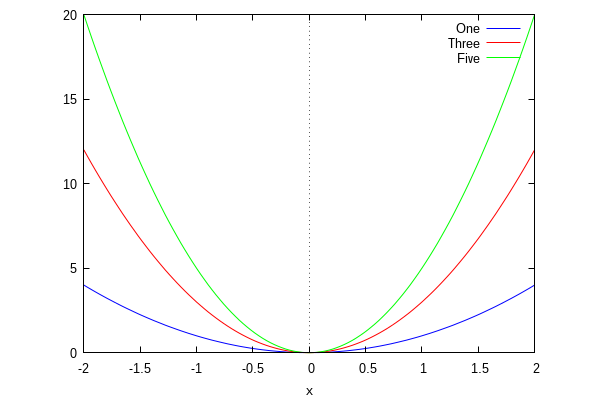
\includegraphics[width=.95\linewidth,height=.80\textheight,keepaspectratio]{Trabajoclase_img/Trabajoclase_4}\mbox{}\]
\[\displaystyle
\]
\[\tag{\%{}o34}\label{o34} 
\mbox{}
\]
%%%%%%%%%%%%%%%
De igual manera también podemos agregar etiquetas a cada eje y título por igual. [xlabel,"nombre"], [ylabel,"nombre"], [legend,"nombre1","nombre 2","nombren"], [title, "Título"] 


\noindent
%%%%%%%%%%%%%%%
%%% INPUT:
\begin{minipage}[t]{8ex}\color{red}\bf
--\ensuremath{\ensuremath{>}}  
\end{minipage}
\begin{minipage}[t]{\textwidth}\color{blue}
 wxplot2d([-16*t\^{}2 - 32*t+50,-16*t\^{}2 - 20*t + 50, -16*t\^{}2 + 50],
   [t,0,2],
   [xlabel,"Time (t) in seconds"],
   [ylabel,"Height in ft"],
[legend,"Fast throw","Medium Throw","Dropped"],
[title, "Different Drop Models"]);
\end{minipage}
%%% OUTPUT:
\[\displaystyle
\tag{\%{}t35}\label{t35} 
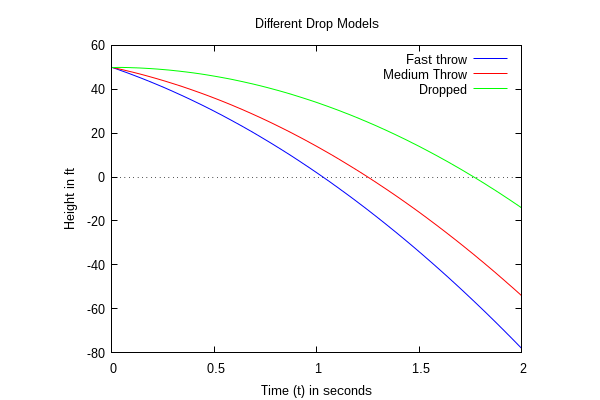
\includegraphics[width=.95\linewidth,height=.80\textheight,keepaspectratio]{Trabajoclase_img/Trabajoclase_5}\mbox{}\]
\[\displaystyle
\]
\[\tag{\%{}o35}\label{o35} 
\mbox{}
\]
%%%%%%%%%%%%%%%
También podemos ajustar el límite referente a la altura de igual forma que con el eje x 


\noindent
%%%%%%%%%%%%%%%
%%% INPUT:
\begin{minipage}[t]{8ex}\color{red}\bf
--\ensuremath{\ensuremath{>}}  
\end{minipage}
\begin{minipage}[t]{\textwidth}\color{blue}
 wxplot2d([-16*t\^{}2 - 32*t+50,-16*t\^{}2 - 20*t + 50, -16*t\^{}2 + 50],
   [t,0,2],
   [y,0,55],
   [xlabel,"Time (t) in seconds"],
   [ylabel,"Height in ft"],
[legend,"Fast throw","Medium Throw","Dropped"],
[title, "Different Drop Models"]);
\end{minipage}
%%% OUTPUT:
\[\displaystyle
\mbox{}\\\mbox{plot2d: some values were clipped.}\mbox{}\\\mbox{plot2d: some values were clipped.}\mbox{}\\\mbox{plot2d: some values were clipped.}\mbox{}\]
\[\displaystyle
\]
\[\tag{\%{}t36}\label{t36} 
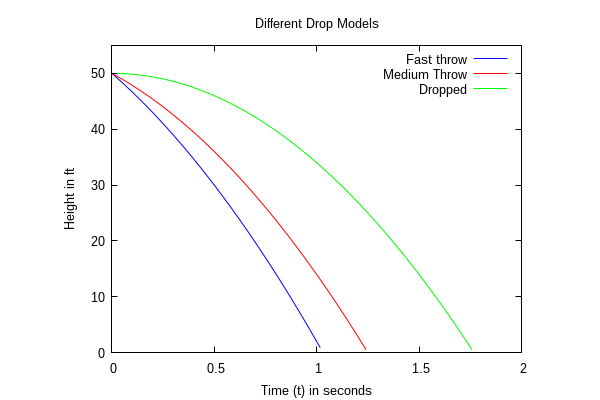
\includegraphics[width=.95\linewidth,height=.80\textheight,keepaspectratio]{Trabajoclase_img/Trabajoclase_6}\mbox{}\]
\[\displaystyle
\]
\[\tag{\%{}o36}\label{o36} 
\mbox{}
\]
%%%%%%%%%%%%%%%

\subsubsection{Asíntotas}

Máxima tiene la facilidad de graficar las asíntotas por su propia cuenta. 


\noindent
%%%%%%%%%%%%%%%
%%% INPUT:
\begin{minipage}[t]{8ex}\color{red}\bf
(\%{}i1) 
\end{minipage}
\begin{minipage}[t]{\textwidth}\color{blue}
 wxplot2d(1/(x-1),
   [x,0,2],
   [y,-10,10],
   [title,"A Graph with Asymptote at x=1"])\$
\end{minipage}
%%% OUTPUT:
\[\displaystyle
\mbox{}\\\mbox{plot2d: expression evaluates to non-numeric value somewhere in plotting range.}\mbox{}\\\mbox{plot2d: some values were clipped.}\mbox{}\]
\[\displaystyle
\]
\[\tag{\%{}t1}\label{t1} 
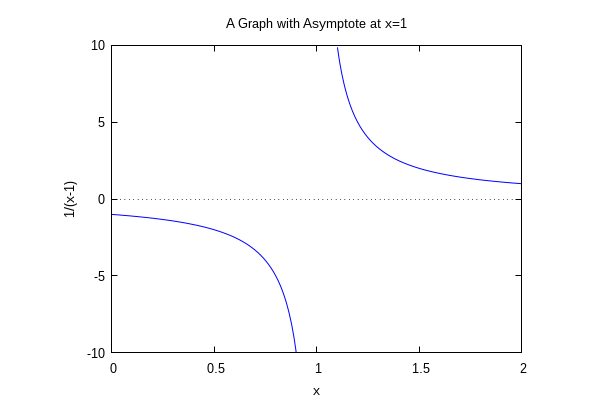
\includegraphics[width=.95\linewidth,height=.80\textheight,keepaspectratio]{Trabajoclase_img/Trabajoclase_7}\mbox{}
\]
%%%%%%%%%%%%%%%
Graficar partes de una ecuación 


\noindent
%%%%%%%%%%%%%%%
%%% INPUT:
\begin{minipage}[t]{8ex}\color{red}\bf
(\%{}i2) 
\end{minipage}
\begin{minipage}[t]{\textwidth}\color{blue}
 E:x\^{}2 -4*x = 5*x\^{}5 + 3*x\^{}2 + 7;
\end{minipage}
%%% OUTPUT:
\[\displaystyle
\tag{E}\label{E}
{{x}^{2}}-4x=5{{x}^{5}}+3{{x}^{2}}+7\mbox{}
\]
%%%%%%%%%%%%%%%


\noindent
%%%%%%%%%%%%%%%
%%% INPUT:
\begin{minipage}[t]{8ex}\color{red}\bf
(\%{}i3) 
\end{minipage}
\begin{minipage}[t]{\textwidth}\color{blue}
    wxplot2d([rhs(E),lhs(E)],
   [x,-5,5],
   [y,-20,20],
   [title,"Two Sides of an Equation"],
   [legend,"Right Side","Left Side"])\$
\end{minipage}
%%% OUTPUT:
\[\displaystyle
\mbox{}\\\mbox{plot2d: some values were clipped.}\mbox{}\\\mbox{plot2d: some values were clipped.}\mbox{}\]
\[\displaystyle
\]
\[\tag{\%{}t3}\label{t3} 
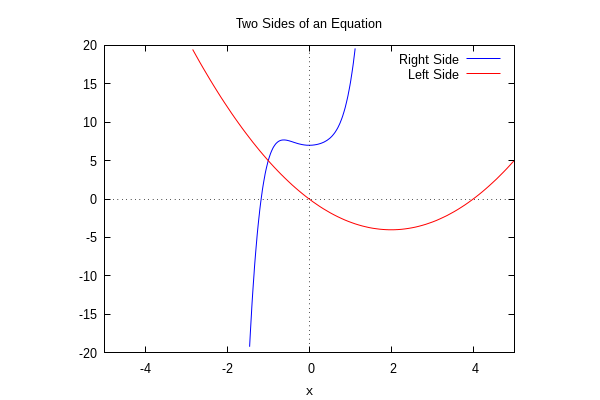
\includegraphics[width=.95\linewidth,height=.80\textheight,keepaspectratio]{Trabajoclase_img/Trabajoclase_8}\mbox{}
\]
%%%%%%%%%%%%%%%
\end{document}
